\documentclass[10pt,leqno]{article}

\usepackage[%
  tmargin=1.2in,bmargin=1.2in,%
  lmargin=1.8in,rmargin=1.8in,%
]{geometry}
\usepackage{fancyhdr}
\usepackage{titlesec}
\usepackage{appendix}
\usepackage{microtype}
\usepackage[hyphens]{url}
\usepackage{enumitem}
\usepackage{xspace}
\usepackage{etoolbox}
\usepackage{ifthen}
\usepackage{tikz}
\usepackage{tikz-cd}

\usepackage{amsmath}
\definecolor{darkred}{rgb}{0.5,0.0,0.0}
\usepackage[%
  colorlinks,%
  linkcolor=darkred,%
  citecolor=darkred,%
  urlcolor=darkred,%
]{hyperref}
\usepackage{amsthm,amssymb}
% \usepackage[lining,semibold]{libertine}
% \usepackage{textcomp,stmaryrd}
% \usepackage[libertine,cmintegrals,bigdelims]{newtxmath}
% \useosf
% \usepackage[%
%   cal=boondox, calscaled=0.97,%
%   bb=boondox, bbscaled=0.98,%
% ]{mathalfa}
\usepackage{cleveref}

\frenchspacing
\urlstyle{rm}

\AtBeginDocument{%
  \setlength{\abovedisplayskip}{1.5ex plus 0.3ex minus 0.3ex}%
  \setlength{\abovedisplayshortskip}{1.0ex plus 0.3ex minus 0.3ex}%
  \setlength{\belowdisplayskip}{1.5ex plus 0.3ex minus 0.3ex}%
  \setlength{\belowdisplayshortskip}{1.0ex plus 0.3ex minus 0.3ex}%
}

\let\theoldbibliography\thebibliography
\renewcommand{\thebibliography}[1]{%
  \theoldbibliography{#1}%
  \setlength{\parskip}{0ex}
  \setlength{\itemsep}{0.5ex plus 0.2ex minus 0.2ex}
  \small
}

\pagestyle{fancy}
\renewcommand{\headrulewidth}{0pt}
\renewcommand{\footrulewidth}{0pt}
\fancyhf{}
\fancyfoot[C]{\small\thepage}

\renewcommand{\title}[1]{\newcommand{\thetitle}{#1}}
\renewcommand{\author}[1]{\newcommand{\theauthor}{#1}}
\renewcommand{\date}[1]{\newcommand{\thedate}{#1}}

\renewcommand{\maketitle}{%
  \begin{center}
    {\bfseries\MakeUppercase{%
      \thetitle}}\\[2.5ex]
    {\footnotesize\MakeUppercase{%
      \theauthor}}\\[2.5ex]
    \ifthenelse{\equal{\thedate}{}}{}{%
      \small%
      \setlength{\tabcolsep}{0.2em}%
      \begin{tabular}{rl}
        original: & \thedate \\
        updated: & \today
      \end{tabular}
    }
  \end{center}
  \vspace{2.5ex}
  \thispagestyle{fancy}
}

%%%%%%%%%%%%%%%%%%%%%%%%%%%%%%%%%%%%%%%%%%%%%%%%%%%%%%%%%%%%%%%%%%%%%%

\cspreto{section}{\setcounter{equation}{0}}

\titleformat{\section}{\centering\scshape}{\thesection.}{0.4em}{}
\titlespacing{\section}{0pt}{*4}{*1}
\titleformat{\subsection}{\scshape}{\thesubsection.}{0.4em}{}
\titlespacing{\subsection}{0pt}{*2.5}{*1}

% Display format for equations
\newcommand{\crefeqfmt}[1]{
  \crefformat{#1}{(##2##1##3)}
  \Crefformat{#1}{(##2##1##3)}
  \crefrangeformat{#1}{(##3##1##4--##5##2##6)}
  \Crefrangeformat{#1}{(##3##1##4--##5##2##6)}
  \crefmultiformat{#1}{(##2##1##3}{, ##2##1##3)}{, ##2##1##3}{, ##2##1##3)}
  \Crefmultiformat{#1}{(##2##1##3}{, ##2##1##3)}{, ##2##1##3}{, ##2##1##3)}
  \crefrangemultiformat{#1}{(##3##1##4--##5##2##6}{, ##3##1##4--##5##2##6)}{, ##3##1##4--##5##2##6}{, ##3##1##4--##5##2##6)}
  \Crefrangemultiformat{#1}{(##3##1##4--##5##2##6}{, ##3##1##4--##5##2##6)}{, ##3##1##4--##5##2##6}{, ##3##1##4--##5##2##6)}
}
% Display format for sections
\newcommand{\crefsecfmt}[1]{%
  \crefformat{#1}{\S##2##1##3}
  \Crefformat{#1}{\S##2##1##3}
  \crefrangeformat{#1}{\S\S##3##1##4--##5##2##6}
  \Crefrangeformat{#1}{\S\S##3##1##4--##5##2##6}
  \crefmultiformat{#1}{\S\S##2##1##3}{ and~##2##1##3}{, ##2##1##3}{ and~##2##1##3}
  \Crefmultiformat{#1}{\S\S##2##1##3}{ and~##2##1##3}{, ##2##1##3}{ and~##2##1##3}
  \crefrangemultiformat{#1}{\S\S##3##1##4--##5##2##6}{ and~##3##1##4--##5##2##6}{, ##3##1##4--##5##2##6}{ and~##3##1##4--##5##2##6}
  \Crefrangemultiformat{#1}{\S\S##3##1##4--##5##2##6}{ and~##3##1##4--##5##2##6}{, ##3##1##4--##5##2##6}{ and~##3##1##4--##5##2##6}
}
\crefeqfmt{equation}
\crefeqfmt{enumi}
\crefeqfmt{enumii}
\crefsecfmt{section}
\crefsecfmt{subsection}
\crefsecfmt{appendix}
\crefname{part}{Part}{Parts}
\crefname{chapter}{Chapter}{Chapters}
\crefname{figure}{Figure}{Figures}

\makeatletter

\newcommand{\thmnumfont}{\bfseries}
\newcommand{\thmheadfont}{\bfseries}
\newcommand{\thmnotefont}{\bfseries}
\newcommand{\thmhorizspace}{0.4em}

\def\swappedhead#1#2#3{%
  \thmnumber{\@upn{{\thmnumfont#2}}\@ifnotempty{#1}{.\hspace{0.25em}}}%
  \thmheadfont\thmname{#1}%
  \@ifnotempty{#3}{\ \thmnote{\thmnotefont(#3)}}%
}
\swapnumbers

\newtheoremstyle{block}%
  {2.0ex plus 0.2ex minus 0.1ex}% Space above
  {2.0ex plus 0.2ex minus 0.1ex}% Space below
  {} % Body font
  {} % Indent amount
  {\thmheadfont} % Theorem head font
  {.} % Punctuation after theorem head
  {\thmhorizspace} % Space after theorem head
  {} % Theorem head spec (can be left empty, meaning ‘normal’)

\renewenvironment{proof}[1][Proof]{\par
  \pushQED{\qed}%
  \normalfont%
  \topsep1ex plus 0.2ex minus 0.1ex\relax%
  \labelsep \thmhorizspace\relax%
  \trivlist
  \item[\hskip\labelsep\thmheadfont
    #1\@addpunct{.}]\ignorespaces
}{%
  \popQED\endtrivlist\@endpefalse%
}

\makeatother

\theoremstyle{block}

\newcommand{\defthm}[2]{%
  \newtheorem{#1}[equation]{#2}%
  \crefeqfmt{#1}%
  \newtheorem*{#1*}{#2}%
}

\defthm{algorithm}{Algorithm}
\defthm{conjecture}{Conjecture}
\defthm{construction}{Construction}
\defthm{convention}{Convention}
\defthm{corollary}{Corollary}
\defthm{definition}{Definition}
\defthm{definitions}{Definitions}
\defthm{example}{Example}
\defthm{examples}{Examples}
\defthm{exercise}{Exercise}
\defthm{fact}{Fact}
\defthm{intuition}{Intuition}
\defthm{lemma}{Lemma}
\defthm{notation}{Notation}
\defthm{nothing}{}
\defthm{proposition}{Proposition}
\defthm{question}{Question}
\defthm{remark}{Remark}
\defthm{remarks}{Remarks}
\defthm{situtation}{Situation}
\defthm{theorem}{Theorem}

\setlist{%
  leftmargin=2.5em, parsep=0ex, listparindent=\parindent,
  itemsep=1.0ex, topsep=1.0ex,%
}

\setlist[enumerate, 1]{%
  label=(\alph*),%
  ref=\alph*,%
  widest=d,%
}
\setlist[enumerate, 2]{%
  label=(\roman*),%
  ref=\theenumi.\roman*,%
}
\setlist[itemize, 1]{%
  label=$\vcenter{\hbox{\footnotesize$\bullet$}}$,%
}
\setlist[itemize, 2]{label=--}

%%%%%%%%%%%%%%%%%%%%%%%%%%%%%%%%%%%%%%%%%%%%%%%%%%%%%%%%%%%%%%%%%%%%%%

\makeatletter

\let\ea\expandafter

\newcount\foreachcount

\def\foreachletter#1#2#3{\foreachcount=#1
  \ea\loop\ea\ea\ea#3\@alph\foreachcount
  \advance\foreachcount by 1
  \ifnum\foreachcount<#2\repeat}

\def\foreachLetter#1#2#3{\foreachcount=#1
  \ea\loop\ea\ea\ea#3\@Alph\foreachcount
  \advance\foreachcount by 1
  \ifnum\foreachcount<#2\repeat}

% Roman: \rA is \mathrm{A}
\def\definerm#1{%
  \ea\gdef\csname r#1\endcsname{\ensuremath{\mathrm{#1}}\xspace}}
\foreachLetter{1}{27}{\definerm}
\foreachletter{1}{27}{\definerm}
% Script: \sA is \mathscr{A}
\def\definescr#1{%
  \ea\gdef\csname s#1\endcsname{\ensuremath{\mathscr{#1}}\xspace}}
\foreachLetter{1}{27}{\definescr}
% Calligraphic: \cA is \mathcal{A}
\def\definecal#1{%
  \ea\gdef\csname c#1\endcsname{\ensuremath{\mathcal{#1}}\xspace}}
\foreachLetter{1}{27}{\definecal}
% Bold: \bA is \mathbf{A}
\def\definebold#1{%
  \ea\gdef\csname b#1\endcsname{\ensuremath{\mathbf{#1}}\xspace}}
\foreachLetter{1}{27}{\definebold}
% Blackboard Bold: \lA is \mathbb{A}
\def\definebb#1{%
  \ea\gdef\csname l#1\endcsname{\ensuremath{\mathbb{#1}}\xspace}}
\foreachLetter{1}{27}{\definebb}
% Fraktur: \ka is \mathfrak{a}, \kA is \mathfrak{A}
\def\definefrak#1{%
  \ea\gdef\csname k#1\endcsname{\ensuremath{\mathfrak{#1}}\xspace}}
\foreachletter{1}{27}{\definefrak}
\foreachLetter{1}{27}{\definefrak}
% Sans serif: \iA \is \mathsf{A}
\def\definesf#1{%
  \ea\gdef\csname i#1\endcsname{\ensuremath{\mathsf{#1}}\xspace}}
\foreachletter{1}{6}{\definesf}
\foreachletter{7}{14}{\definesf}
\foreachletter{15}{27}{\definesf}
\foreachLetter{1}{27}{\definesf}
% Bar: \Abar is \overline{A}, \abar is \overline{a}
\def\definebar#1{%
  \ea\gdef\csname #1bar\endcsname{\ensuremath{\overline{#1}}\xspace}}
\foreachLetter{1}{27}{\definebar}
\foreachletter{1}{8}{\definebar} % \hbar is something else!
\foreachletter{9}{15}{\definebar} % \obar is something else!
\foreachletter{16}{27}{\definebar}
% Tilde: \Atil is \widetilde{A}, \atil is \widetilde{a}
\def\definetil#1{%
  \ea\gdef\csname #1til\endcsname{\ensuremath{\widetilde{#1}}\xspace}}
\foreachLetter{1}{27}{\definetil}
\foreachletter{1}{27}{\definetil}
% Hats: \Ahat is \widehat{A}, \ahat is \widehat{a}
\def\definehat#1{%
  \ea\gdef\csname #1hat\endcsname{\ensuremath{\widehat{#1}}\xspace}}
\foreachLetter{1}{27}{\definehat}
\foreachletter{1}{27}{\definehat}
% Checks: \Achk is \widecheck{A}, \achk is \widecheck{a}
\def\definechk#1{%
  \ea\gdef\csname #1chk\endcsname{\ensuremath{\widecheck{#1}}\xspace}}
\foreachLetter{1}{27}{\definechk}
\foreachletter{1}{27}{\definechk}
% Underline: \Aund is \underline{A}, \aund is \underline{a}
\def\defineul#1{%
  \ea\gdef\csname #1und\endcsname{\ensuremath{\underline{#1}}\xspace}}
\foreachLetter{1}{27}{\defineul}
\foreachletter{1}{27}{\defineul}

\makeatother

%%%%%%%%%%%%%%%%%%%%%%%%%%%%%%%%%%%%%%%%%%%%%%%%%%%%%%%%%%%%%%%%%%%%%%

\usetikzlibrary{calc,decorations.pathmorphing,shapes,arrows}
\tikzcdset{
  arrow style=tikz,
  diagrams={>={stealth}},
}

\newcommand{\arrlen}{1em}
\renewcommand{\to}{\mathrel{\tikz[baseline]%
    \draw[>=stealth,->](0,0.5ex)--(\arrlen,0.5ex);}}
\newcommand{\from}{\mathrel{\tikz[baseline]%
    \draw[>=stealth,<-](0,0.5ex)--(\arrlen,0.5ex);}}
\renewcommand{\mapsto}{\mathrel{\tikz[baseline]%
    \draw[>=stealth,|->](0,0.5ex)--(\arrlen,0.5ex);}}
\newcommand{\inj}{\mathrel{\tikz[baseline]%
    \draw[>=stealth,right hook->](0,0.5ex)--(\arrlen,0.5ex);}}
\newcommand{\surj}{\mathrel{\tikz[baseline]%
    \draw[>=stealth,->>](0,0.5ex)--(\arrlen,0.5ex);}}
\newcommand{\fromto}{\mathrel{%
  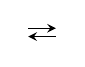
\begin{tikzpicture}[baseline]%
    \draw[>=stealth,<-](0,0.15ex)--(\arrlen,0.15ex);%
    \draw[>=stealth,->](0,0.85ex)--(\arrlen,0.85ex);%
  \end{tikzpicture}}}
\newcommand{\doubto}{\mathrel{%
  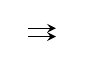
\begin{tikzpicture}[baseline]%
    \draw[>=stealth,->](0,0.15ex)--(\arrlen,0.15ex);%
    \draw[>=stealth,->](0,0.85ex)--(\arrlen,0.85ex);%
  \end{tikzpicture}}}
\newcommand{\lblto}[1]{\mathrel{%
    \begin{tikzpicture}[baseline= {( $ (current bounding box.south) + (0,-0.5ex) $ )}]
      \node[inner sep=.4ex] (a) {\,$\scriptstyle #1$\,};
      \draw[>=stealth,->] (a.south west) -- (a.south east);
    \end{tikzpicture}}}
\newcommand{\isoto}{\lblto{\sim}}

\newcommand{\simpl}[3]{
  \begin{tikzcd}[ampersand replacement=\&, column sep=small]
    #1 \&
    #2 \ar[l, shift right=0.35ex]
       \ar[l, shift left=0.35ex] \&
    #3 \ar[l, shift right=0.70ex]
       \ar[l, shift left=0.70ex]
       \ar[l] \&
    \cdots \ar[l, shift right=0.35ex]
           \ar[l, shift left=0.35ex]
           \ar[l, shift right=1.05ex]
           \ar[l, shift left=1.05ex]
  \end{tikzcd}
}
\newcommand{\cosimpl}[3]{
  \begin{tikzcd}[ampersand replacement=\&, column sep=small]
    #1 \ar[r, shift right=0.35ex]
       \ar[r, shift left=0.35ex] \&
    #2 \ar[r, shift right=0.70ex]
       \ar[r, shift left=0.70ex]
       \ar[r] \&
    #3 \ar[r, shift right=0.35ex]
       \ar[r, shift left=0.35ex]
       \ar[r, shift right=1.05ex]
       \ar[r, shift left=1.05ex] \&
    \cdots
  \end{tikzcd}
}

\newcommand{\tto}{\mathrel{\tikz[baseline]%
    \draw[>=stealth,->,double, double distance = 0.3ex](0,0.5ex)--(\arrlen,0.5ex);}}
\newcommand{\doubfrom}{\mathrel{%
  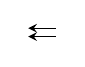
\begin{tikzpicture}[baseline]%
    \draw[>=stealth,<-](0,0.15ex)--(\arrlen,0.15ex);%
    \draw[>=stealth,<-](0,0.85ex)--(\arrlen,0.85ex);%
  \end{tikzpicture}}}
\newcommand{\tripfrom}{\mathrel{%
  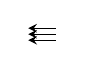
\begin{tikzpicture}[baseline]%
    \draw[>=stealth,<-](0,0.00ex)--(\arrlen,0.00ex);%
    \draw[>=stealth,<-](0,0.50ex)--(\arrlen,0.50ex);%
    \draw[>=stealth,<-](0,1.00ex)--(\arrlen,1.00ex);%
  \end{tikzpicture}}}


\renewcommand{\l}{\left}
\renewcommand{\r}{\right}
\newcommand{\f}{\frac}
\renewcommand{\o}{\overline}
\renewcommand{\u}{\underline}
\newcommand{\til}{\widetilde}
\renewcommand{\hat}{\widehat}
\newcommand{\del}{\partial}
\newcommand{\dash}{\text{-}}
\renewcommand{\c}{\colon}
\newcommand{\lc}{\,:\!}
\newcommand{\ce}{\coloneq}%{\mathrel{:=}}
\newcommand{\ec}{\eqcolon}%{\mathrel{=:}}
\newcommand{\iso}{\simeq}
\newcommand{\dual}{\vee}
\newcommand{\ldb}{\llbracket}
\newcommand{\rdb}{\rrbracket}

\newcommand{\Obj}{\operatorname{Obj}}
\newcommand{\Hom}{\operatorname{Hom}}
\newcommand{\Map}{\operatorname{Map}}
\newcommand{\Fun}{\operatorname{Fun}}
\newcommand{\Aut}{\operatorname{Aut}}
\newcommand{\Iso}{\operatorname{Iso}}
\renewcommand{\id}{\mathrm{id}}
\renewcommand{\im}{\operatorname{im}}
\newcommand{\op}{\mathrm{op}}
\newcommand{\univ}{\mathrm{univ}}
\newcommand{\colim}{\operatorname*{colim}}
\newcommand{\dlim}{\displaystyle\lim}
\newcommand{\dcolim}{\displaystyle\colim}
\newcommand{\Spec}{\operatorname{Spec}}
\newcommand{\Spf}{\operatorname{Spf}}

%%%%%%%%%%%%%%%%%%%%%%%%%%%%%%%%%%%%%%%%%%%%%%%%%%%%%%%%%%%%%%%%%%%%%%


\title{Grand unification of cohomology}
\author{Arpon Raksit}
\date{February 16, 2016}

\numberwithin{block}{section}
\addtocounter{section}{-1}
% \cspreto{section}{\setcounter{equation}{0}}

\begin{document}
\maketitle

%%%%%%%%%%%%%%%%%%%%%%%%%%%%%%%%%%%%%%%%%%%%%%%%%%%%%%%%%%%%%%%%%%%%%%

\newcommand{\AbGroups}{\mathrm{AbGroups}}
\newcommand{\fin}{\mathrm{fin}}
\newcommand{\Ho}{\operatorname{Ho}}
\newcommand{\Push}{\operatorname{Push}}
\newcommand{\sing}{\mathrm{sing}}
\newcommand{\Spaces}{\mathrm{Spaces}}

%%%%%%%%%%%%%%%%%%%%%%%%%%%%%%%%%%%%%%%%%%%%%%%%%%%%%%%%%%%%%%%%%%%%%%

\section{Introduction}

The words ``homology'' and ``cohomology'' are ubiquitous in modern topology, geometry, and algebra. What do they mean?

In algebraic topology we are introduced to singular homology and cohomology, and then perhaps to other ``generalized'' cohomology theories like the (topological) K-theories and bordism theories. In complex and algebraic geometry we are introduced to sheaf cohomology, concretely as \v{C}ech cohomology, and more axiomatically in the framework of derived functors. And in algebra and number theory one runs into group homology and cohomology, which similarly have concrete characterizations in addition to fitting into the framework of derived functors.

So, how are all these notions of homology and cohomology are related? Why do they deserve the same name? The theory of derived functors accounts for quite a bit, but how is it related to something like topological K-theory? The ultimate goal of this note is to explain one possible answer to these questions, which is that there is indeed a common framework for all of these notions, in terms of ``sheaves of spectra''; we'll get to this in \cref{unify}. Before that we will give introductions to these notions of homology and cohomology; topology is in \cref{topology}, geometry and algebra in \cref{geometry}. With a view towards unification, these introductions come from an uncompromisingly homotopy-theoretic\footnote{And therefore totally ahistorical, I should probably note.} perspective. We thus begin in \cref{primer} with a sketchy, philisophical guide on homotopical mathematics.

%%%%%%%%%%%%%%%%%%%%%%%%%%%%%%%%%%%%%%%%%%%%%%%%%%%%%%%%%%%%%%%%%%%%%%

\section{A primer on homotopical thinking}
\label{primer}

Things to talk about:
\begin{itemize}
\item Homotopy coherence / data vs. conditions (gluing bundles / stacks?)
\item (Co)fiber sequences (and I guess (co)limits)
\item The $\infty$-categories of spaces (free cocompletion)
\item The $\infty$-category of chain complexes (stable $\infty$-categories, triangulated categories, t-structures...).
\end{itemize}

%%%%%%%%%%%%%%%%%%%%%%%%%%%%%%%%%%%%%%%%%%%%%%%%%%%%%%%%%%%%%%%%%%%%%%

\section{Topology: Eilenberg-Steenrod and spectra}
\label{topology}

\begin{nothing}
  \label{topology-spiel}
  The central goal of algebraic topology is to learn about spaces\footnote{Classically this means topological spaces up to weak homotopy equivalence, but we can just take this to mean objects of the $\infty$-category of $\Spaces$.} by constructing and analyzing algebraic invariants of them. Precisely, an ``algebraic invariant'' should be a functor $\Spaces \to \sA$ (or $\Spaces^\op \to \sA$), where $\sA$ is some kind of ``algebraic'' category we can get our hands on, e.g. the categories of groups or rings, or perhaps quasi-coherent sheaves on some algebro-geometric object. For this to be fruitful, we'd like to find invariants that both:
  \begin{enumerate}
  \item contain interesting information;
  \item are readily computable.
  \end{enumerate}
  These desiderata are of course in tension with each other. For example, the homotopy group functors $X \goesto \pi_*(X)$ in some sense encode all information in spaces, but are incredibly difficult to compute. Nevertheless, various invariants that are simultaneously interesting and computable have been found; they're what make algebraic topology worthwhile!

  \emph{Cohomology theories} give one class of interesting but computable invariants. In fact, we will introduce them here from an axiomatic perspective, due to Eilenberg and Steenrod, that essentially says: cohomology theories are invariants satisfying some axioms ensuring they are somewhat computable.

  The main axiom we will impose is a kind of \emph{locality}. Let's discuss this. Suppose we have an invariant of spaces $E \c \Spaces^\op \to \sA$ (cohomology theories are contravariant so let's start thinking that way from the start), and we want to compute $E(X)$ for some space $X$. It's often the case that we can break $X$ up into smaller pieces $\{U_i\}$ that are easier to understand; e.g., if $X$ is the underlying space of a manifold, then $X$ can be covered by pieces equivalent to $\bR^n$, hence equivalent to a point. It would be nice if $E$ was of a ``local'' nature, so that knowing the pieces $E(U_i)$ would allow us to compute $E(X)$. Of course, the word ``compute'' might mean anything, and indeed the form it takes in the definition of cohomology theory probably isn't the first thing you'd think of. To partially justify this, let's see why the thing you actually might think of first wouldn't make for a great definition.

  The categorical/homotopical way to speak about being broken into pieces is via the notion of pushout. Namely, we think of a space $X$ as being the ``gluing'' of two spaces $U_1$ and $U_2$ along a third space $U_{1,2}$ when we are given a pushout square
  \[
    \begin{tikzcd}
      U_{1,2} \ar[r, "i_1"] \ar[d, "i_2", swap] &
      U_1 \ar[d, "j_1"] \\
      U_2 \ar[r, "j_2"] &
      X
    \end{tikzcd}
  \]
  in the $\infty$-category $\Spaces$. Let's take the target category $\sA$ of $E$ to be any abelian (discrete) category.\footnote{Feel free to just take $\sA$ to be the category of abelian groups. We'll be focusing on this case shortly anyways.} Then, recalling that we're in a contravariant situation, this pushout square determines a sequence of maps
  \[
    E(X) \lblto{(E(j_1),-E(j_2))}
    E(U_1) \oplus E(U_2) \lblto{E(i_1) + E(i_2)}
    E(U_{1,2});
  \]
  and since $j_1i_1 \iso j_2i_2 \implies E(i_1)E(j_1) = E(i_2)E(j_2)$, we see that the composite of these maps is zero. Thus, if we'd like to recover $E(X)$ from $E(U_1)$, $E(U_2)$, and $E(U_{1,2})$, we might first think to ask that this sequence be a short exact one.

  However, I claim that any invariant satisfying this strong locality property (and valued in an abelian category) isn't too interesting. Namely, given any space $Y$, suppose we take $U_{1,2} = Y$ and $U_1 = \pt = U_2$, so that $X \iso \Sigma Y$, and suppose we get a short-exact sequence
  \[
    0 \to E(X) \lblto{\alpha} E(\pt) \oplus E(\pt) \lblto{\beta} E(Y) \to 0
  \]
  from the above. Now, in addition to the maps $j_1,j_2 \c \pt \to X$, we have our canonical map $p \c X \to \pt$; these maps satisfy $pj_1 \iso \id_\pt \iso pj_2$, and hence we get $E(j_1)E(p) = \id_{E(\pt)} = E(j_2)E(p)$. This implies $E(j_1),E(j_2)$ must be surjective, and hence $\alpha$ is surjective. By exactness in the middle it follows that $\beta = 0$, and by exactness on the right this means $E(Y) \iso 0$. Thus $E$ takes every space to $0$; hopefully we can agree that this won't be too useful.

  Observe, though, that it was really the requirement of right-exactness that trivialized the situation above, and that left-exactness really played no role. So what if we just demand that the sequence be exact in the middle? It turns out that this is much more reasonable. However, once we relax to this situation, it's natural to demand something else. Namely, we'd like to systematically understand the ``failure'' of the sequence to be short-exact; one precise way to achieve this would be to extend the sequence on both sides, i.e. to put in the context of a long(er) exact sequence. This finally motivates the following definition of cohomology theories.\footnote{Of course, while I find this motivation conceptually satisfying, it is somewhat artificial. The true motivation for the definition of cohomology theory is the fact that ``nature'' contains many interesting examples!}
\end{nothing}

\begin{nothing}
  \label{cohomology-theory}
  Let $\sC$ be a $\infty$-category admitting finite colimits (the primary example of interest is $\sC = \Spaces$, but allowing for some variations here, e.g. $\sC = \Spaces^\fin$, will be useful).

  \begin{subnotation*}
    \label{pushout-category}
    Let $\Push(\sC)$ denote the $\infty$-category of pushout squares in $\sC$ (i.e. take the diagram category of squares in $\sC$, and then restrict to the full subcategory of pushout squares).

    Let $\rI \c \Push(\sC) \to \sC$ denote the functor taking a pushout square to its initial object (i.e. the object we ``glue along''), and $\rF \c \Push(\sC) \to \sC$ the functor taking a pushout square to its final object (i.e. the actual pushout, or ``glued'' object).
  \end{subnotation*}

  \begin{subnotation*}
    \label{abgroups}
    We denote the category of abelian groups by $\AbGroups$.
  \end{subnotation*}

  \begin{subdefinition}
    \label{cohomology-theory-def}
    A \defemph{cohomology theory} on $\sC$ is a sequence of functors and natural transformations
    \begin{align*}
      &E^n \c \sC^\op \to \AbGroups,  \\
      &\del^n \c E^n \circ \rI \to E^{n+1} \circ \rF \c \Push(\sC) \to \AbGroups
    \end{align*}
    for $n \in \bZ$ satisfying the following conditions:
    \begin{enumerate}
    \item \label{cohomology-theory-additivity}
      \emph{Additivity}: For any set of objects $\{X_i\}$ that admits a coproduct in $\sC$, the canonical map $H^n(\coprod_i X_i) \to \prod_i H^n(X_i)$ is an isomorphism.
    \item \label{cohomology-theory-locality}
      \emph{Locality}: For any pushout square $\sigma$:
      \[
        \begin{tikzcd}
          U_{1,2} \ar[r, "i_1"] \ar[d, "i_2", swap] &
          U_1 \ar[d, "j_1"] \\
          U_2 \ar[r, "j_2"] &
          X
        \end{tikzcd}
      \]
      in $\sC$, the sequence
      \[
        \cdots \to
        E^{n-1}(U_{1,2}) \lblto{\del^{n-1}}
        E^n(X) \lblto{\alpha^n}
        E^n(U_1) \oplus E(U_2) \lblto{\beta^n}
        E^n(U_{1,2}) \lblto{\del^n}
        E^{n+1}(X) \to
        \cdots
      \]
      is exact, where here $\alpha^n \ce (E^n(j_1),-E^n(j_2))$ and $\beta^n \ce E^n(i_1) + E^n(i_2)$.
    \end{enumerate}
  \end{subdefinition}

  \begin{subremark}
    \label{cohomology-theory-homotopy-factor}
    Note that the functors $E^n$ automatically factor through the homotopy category $\Ho(\sC)^\op$, since $\AbGroups$ is a discrete category.
  \end{subremark}

  \begin{subremark*}
    The locality axiom \cref{cohomology-theory-locality} is usually named after Mayer and Vietoris, and the exact sequence there is referred to as a \emph{Mayer-Vietoris sequence}.
  \end{subremark*}
\end{nothing}

\begin{example}
  \label{singular-cohomology}
  Our first example of a cohomology theory is singular cohomology of spaces with coefficients in an abelian group $A$; the underlying functor is denoted on objects by $X \mapsto \rH^n(X;A)$. I have no desire to recall the explicit construction of singular cohomology or what the relevant boundary maps $\del^n$ are, but I do want to recall that singular cohomology is uniquely characterized by being a cohomology theory together with its values on the spheres $\rS^k$ for $k \ge 0$:
  \[
    \rH^n(\rS^k;A) \iso
    \begin{cases}
      A, & n \in \{0,k\} \\
      0, & \text{otherwise}.
    \end{cases}
  \]
\end{example}

\begin{nothing}
  \label{reducing-cohomology}
  Let $(E^n,\del^n)_{n \in \bZ}$ be a cohomology theory on $\Spaces$. Suppose given a pointed space $i \c \pt \to X$. Let $p \c X \to \pt$ be the canonical map. Then $pi = \id_\pt$, so for each $n \in \bZ$ we get a canonical splitting
  \[
    E^n(X) \iso E^n(\pt) \oplus \Etil^n(X),
  \]
  where $\Etil^n(X) \ce \ker(E^n(i))$. Our next goal is to reformulate the above definition of cohomology theory in terms of these ``reduced'' functors $\Etil^*$ (because it will be illuminating!).

  \begin{subnotation*}
    Let $\sC_\pt$ be a pointed $\infty$-category.\footnote{Note that, for now, the subscript $\pt$ in $\sC_\pt$ is purely decorative, reminding us that we're in the pointed setting. However, we will soon consider the case where $\sC_\pt$ is the $\infty$-category of pointed objects in some $\infty$-category $\sC$, e.g. $\sC = \Spaces$ and $\sC_\star = \Spaces_\pt$ is the $\infty$-category of pointed spaces.} Let $\Sigma \c \sC_\pt \to \sC_\pt$ denote the suspension functor.
  \end{subnotation*}

  \begin{subdefinition}
    \label{reduced-cohomology-theory}
    A \emph{reduced cohomology theory} on $\sC_\pt$ is a sequence of functors and natural isomorphisms
    \begin{align*}
      &\Etil^n \c \sC_*^\op \to \AbGroups, & \\
      &\delta^n \c \Etil^n \isoto \Etil^{n+1} \circ \Sigma\c \sC_\pt^\op \to \AbGroups &
    \end{align*}
    for $n \in\bZ$ satisfying the following conditions:
    \begin{enumerate}
    \item \label{reduced-cohomology-theory-additivity}
      \emph{Additivity}: For any set of objects $\{X_i\}$ in $\sC_\pt$, the canonical map $\Etil^n(\bigvee_i X_i) \to \prod_i \Etil^n(X_i)$ is an isomorphism. Here $\bigvee$ denotes the coproduct in $\sC_\pt$.\footnote{We use $\bigvee$ instead of $\coprod$ to evoke ``wedge sum'', which is what the coproduct is in the case $\sC_\pt = \Spaces_\pt$ (as well as to distinguish it from the coproduct in unpointed categories later on).} 
    \item \label{reduced-cohomology-theory-exactness}
      \emph{Exactness}: For any cofiber sequence $X \to Y \to Z$ in $\sC_\pt$, the induced sequence $\Etil^n(Z) \to \Etil^n(Y) \to \Etil^n(Z)$ is exact for each $n \in \bZ$.
    \end{enumerate}
  \end{subdefinition}

  \begin{subremark}
    \label{reduced-cohomology-theory-homotopy-factor}
    As in the definition of cohomology theory \cref{cohomology-theory-homotopy-factor}, note that the functors $\Etil^n$ automatically factor through the homotopy category $\Ho(\sC_\pt)^\op$.
  \end{subremark}

  \begin{subremark}
    \label{reduced-cohomology-theory-point}
    The additivity axiom \cref{reduced-cohomology-theory-additivity} includes the degenerate case of the empty set of objects, in which case it tells us that $\Etil^n(\pt) \iso 0$ for all $n \in \bZ$.

    This implies that $\Etil^n(h) = 0$ for any nullhomotopic map $h$ in $\sC_\pt$. In particular, if
    \[
      X \lblto{f} Y \lblto{g} Z
    \]
    is a cofiber sequence in $\sC_\pt$, the induced composite $\Etil^n(f)\Etil^n(g) = \Etil^n(gf)$ must be the zero map. Thus, the exactness condition \cref{reduced-cohomology-theory-exactness} is equivalent to requiring only that any element in the kernel of $\Etil^n(f)$ lies in the image of the map $\Etil^n(g)$.
  \end{subremark}

  \begin{subremark}
    \label{reduced-cohomology-theory-full-exactness}
    In comparison to the Mayer-Vietoris sequence appearing in the definition of cohomology theory \cref{cohomology-theory-def}\cref{cohomology-theory-locality}, perhaps the exactness axiom \cref{reduced-cohomology-theory-exactness} here seems too weak: we only demanded a three-term exact sequence at each $n \in \bZ$, rather than a long exact sequence relating all $n$. However, this weakness is an illusion; we in fact automatically get a long exact sequence, as follows.
    
    Suppose given a cofiber sequence
    \[
      X \lblto{f} Y \lblto{g} Z
    \]
    in $\sC_*$. Recall that there is a canonical map $h \c Z \to \Sigma X$, coming from the pasting of pushout squares
    \[
      \begin{tikzcd}
        X \ar[r, "f"] \ar[d] &
        Y \ar[r] \ar[d, "g"] &
        * \ar[d] \\
        * \ar[r] &
        Z \ar[r, "h"] \ar[d] &
        \Sigma X \ar[d, "\Sigma f"] \\
        &
        * \ar[r] &
        \Sigma Y.
      \end{tikzcd}
    \]
    Composing $\Etil^{n+1}(h) \c \Etil^{n+1}(\Sigma X) \to \Etil^{n+1}(Z)$ with $\delta^n \c \Etil^n(X) \isoto \Etil^{n+1}(\Sigma X)$, we obtain a map $\del^n \c \Etil^n(X) \to \Etil^{n+1}(Z)$. This gives us a sequence
    \[
      \cdots \to
      \Etil^{n-1}(X) \lblto{\del^{n-1}}
      \Etil^n(Z) \lblto{\Etil^n(g)}
      \Etil^n(Y) \lblto{\Etil^n(f)}
      \Etil^n(X) \lblto{\del^n}
      \Etil^{n+1}(Z) \to
      \cdots,
    \]
    and in fact it's exact:
    \begin{itemize}
    \item Exactness at $\Etil^n(Y)$ follows from our exactness condition
      applied to the original cofiber sequence $X \lblto{f} Y \lblto{g} Z$.
    \item Exactness at $\Etil^n(Z)$ follows from our exactness condition applied to the cofiber sequence $Y \lblto{g} Z \lblto{h} \Sigma X$.
    \item Exactness at $\Etil^n(X)$ follows from our exactness condition applied to the cofiber sequence $Z \lblto{h} \Sigma X \lblto{\Sigma f} \Sigma Y$.
    \end{itemize}
  \end{subremark}
\end{nothing}


\begin{remarks}
  \label{cohomology-theory-remarks}
  Our definition \cref{cohomology-theory} of cohomology theory merits some commentary. Notation is as in the definition.
  \begin{enumerate}[leftmargin=*]
  \item \label{cohomology-theory-automatically-abelian}
    It would have been equivalent to have taken the functors $H^n$ to be valued only in sets rather than in abelian groups. Indeed, we have isomorphisms $\delta^{n+1} \circ \delta^n \c H^n(X) \isoto H^{n+2}(\Sigma^2 X)$, and since $\Sigma^2 X$ is a commutative cogroup object in $\Ho(\Spaces_*)$, it follows that $H^n(X)$ canonically has the structure of an abelian group object.

    Note also that the identity element $0 \in H^n(X)$ is picked out by the map $0 \iso H^n(*) \to H^n(X)$ induced by the unique map $X \to *$.

  \end{enumerate}
\end{remarks}

%%%%%%%%%%%%%%%%%%%%%%%%%%%%%%%%%%%%%%%%%%%%%%%%%%%%%%%%%%%%%%%%%%%%%%

\section{Geometry \& algebra: derived categories and functors}
\label{geometry}

%%%%%%%%%%%%%%%%%%%%%%%%%%%%%%%%%%%%%%%%%%%%%%%%%%%%%%%%%%%%%%%%%%%%%%

\section{Grand unification: sheaves of spectra}
\label{unify}

%%%%%%%%%%%%%%%%%%%%%%%%%%%%%%%%%%%%%%%%%%%%%%%%%%%%%%%%%%%%%%%%%%%%%%

% \bibliographystyle{amsalpha}
% \bibliography{refs}

\end{document}
